\documentclass[a4paper,10pt]{article}
\usepackage{a4wide}
\usepackage{amsmath}
\usepackage{amssymb}
%\usepackage{empheq}
\usepackage[english]{babel}
\usepackage{graphicx}
\usepackage{enumerate}
\usepackage{subcaption,array}
\usepackage{multicol}
%\usepackage{mathtools}
\usepackage{latexsym}
\usepackage{fullpage}
\usepackage{verbatim}
\usepackage{algorithm}
\usepackage{algpseudocode}
\usepackage{float}
\usepackage{bbm}
\usepackage[section]{placeins} % Prevent floats from passing beyond \FloatBarrier; keep floats within their sections
\usepackage{appendix}
\usepackage{import} %tex bestanden importeren deze moeten alleen tekst bevatten geen \begin{document} etc.
\usepackage{listings}
\usepackage{eurosym}
\usepackage[utf8]{inputenx}
\usepackage{program}
\usepackage{bookmark}

\newcommand{\desda}{\Leftrightarrow}
\newcommand{\rr}{\mathbb{R}}
\newcommand{\nn}{\mathbb{N}}
\newcommand{\zz}{\mathbb{Z}}
\newcommand{\qq}{\mathbb{Q}}
\newcommand{\rn}{\mathbb{R}^n}
\newcommand{\fdr}{f:D\rightarrow \rr}
\newcommand{\ul}{\underline}
\newcommand{\pp}{\mathbb{P}}
\newcommand{\ee}{\mathbb{E}}
\newcommand{\lnn}{\tilde{L}_n}
\newcommand{\convdis}{\overset{d}{\longrightarrow}}



\newcommand{\onaf}{\perp\!\!\!\perp}
\newcommand\red[1]{{\color{red}#1}} %kleurt text rood


\lstset{                         %settings voor code, zie ook http://en.wikibooks.org/wiki/LaTeX/Source_Code_Listings
breaklines=true,                 % sets automatic line breaking
commentstyle=\color{mygreen},    % comment style
%frame=single,                    % adds a frame around the code
keywordstyle=\color{blue},       % keyword style    \bfseries voor Bold
numberstyle=\tiny\color{black}, % the style that is used for the line-numbers
rulecolor=\color{black},         % if not set, the frame-color may be changed on line-breaks within not-black text
numbers=left,                    % where to put the line-numbers; possible values are (none, left, right)
}
\setlength\parindent{0pt}
\renewcommand\lstlistlistingname{Lijst van listings}
\usepackage{color}                  %Voor kleuren, o.a. in code
\usepackage{xcolor}                 %Voor kleuren, werkend krijgen  van box boven code
\definecolor{mygreen}{rgb}{0,0.6,0} %groene kleur voor comments in code
\usepackage{caption}
\DeclareCaptionFont{white}{\color{white}}
%\DeclareCaptionFormat{listing}{\colorbox{gray}{\parbox{\textwidth}{#1#2#3}}}
%\captionsetup[lstlisting]{format=listing,labelfont=white,textfont=white}

\usepackage{fancyhdr} %Footers en Headers
\setlength{\headheight}{15.0 pt}
\setlength{\headsep}{0.5 cm}
\pagestyle{fancy}
\fancyfoot[L]{} %naam van groep
\fancyfoot[C]{}
\fancyfoot[R]{\thepage}
\renewcommand{\footrulewidth}{0.4pt}

\fancyhead[L]{\large{\emph{Advanced simulation}}} %Naam van project
\fancyhead[C]{}
\renewcommand{\headrulewidth}{0pt} %thickness of the decorative lines on the header

\usepackage{hyperref}


\setcounter{secnumdepth}{4}% hoever de secties doornummeren
\setcounter{tocdepth}{3} %hoever de inhoudsopgave doornummert


%\setcounter{lofdepth}{2} %hoever de list of figures doornummert
%\setcounter{lotdepth}{2} % hoever de list of tables doornummert
\begin{document}
%\pagenumbering{roman}
\begin{titlepage}

\newcommand{\HRule}{\rule{\linewidth}{0.5mm}} % Defines a new command for the horizontal lines, change thickness here

\centering % Center everything on the page

%----------------------------------------------------------------------------------------
%	TITLE SECTION
%----------------------------------------------------------------------------------------
\HRule \\[0.4cm]
{ \Huge \bfseries Algorithm primitives}\\[0.4cm] % Title of your document
\HRule \\[1.5cm]

%----------------------------------------------------------------------------------------
%	HEADING SECTIONS
%----------------------------------------------------------------------------------------

%\textsc{\LARGE Technische universiteit Eindhoven}\\[1.5cm] % Name of your university/college
\textsc{\large Master Thesis}\\[1.0cm] % Minor heading such as course title vakcode
%----------------------------------------------------------------------------------------
%	LOGO SECTION
%----------------------------------------------------------------------------------------

%\fbox{\includegraphics[width=0.8\textwidth]{bus.png}}\\[1cm] % Include a department/university logo - this will require the graphicx package

%----------------------------------------------------------------------------------------
%	AUTHOR SECTION
%----------------------------------------------------------------------------------------
\vfill % Fill the rest of the page with whitespace
% Alles onder elkaar

L.D. Stooker, 0819041 \\ [1cm]


%----------------------------------------------------------------------------------------
%	DATE SECTION
%----------------------------------------------------------------------------------------

{\large \today}\\[3cm] % Date, change the \today to a set date if you want to be precise



%----------------------------------------------------------------------------------------



\end{titlepage}

\begin{abstract}
To improve existing automated picking of a machine learning algorithm

\end{abstract}

\newpage
\tableofcontents
\newpage


\section{Introduction} \label{Chapter1}
This report is the result of my graduation project which completes my Business Information Systems study at Eindhoven University of Technology.
The project was performed internally at the University in the Data mining department.
In this project we investigated annotations of primitives, more specifically primitives in the scikit-learn library.
In the section \ref{Intr-Prob} we will briefly explain more about primitives and the annotations.
To elaborate on this we will outline the research questions and thesis structure
 

\subsection{problem description}\label{Intr-Prob}
Machine learning is a growing field that can help process the increase of available data\cite{Big-data}\cite{ML-trends}. 
Python is a language which holds premade machine learning algorithms in libraries like scikit-learn\cite{scikit-learn}.
In recent years python is also increasing in so called market share for machine learning\cite{python-pop}.
To help machine learners using the scikit-learn library made a model to indicate what algorithm to use for what problem. 
In figure \ref{fig:FlowChartML} you can see that depending on size of the data and early results different algorithms are recommend.
 

\begin{figure}[h] %use t for top of page instead of h for here
	\centering
	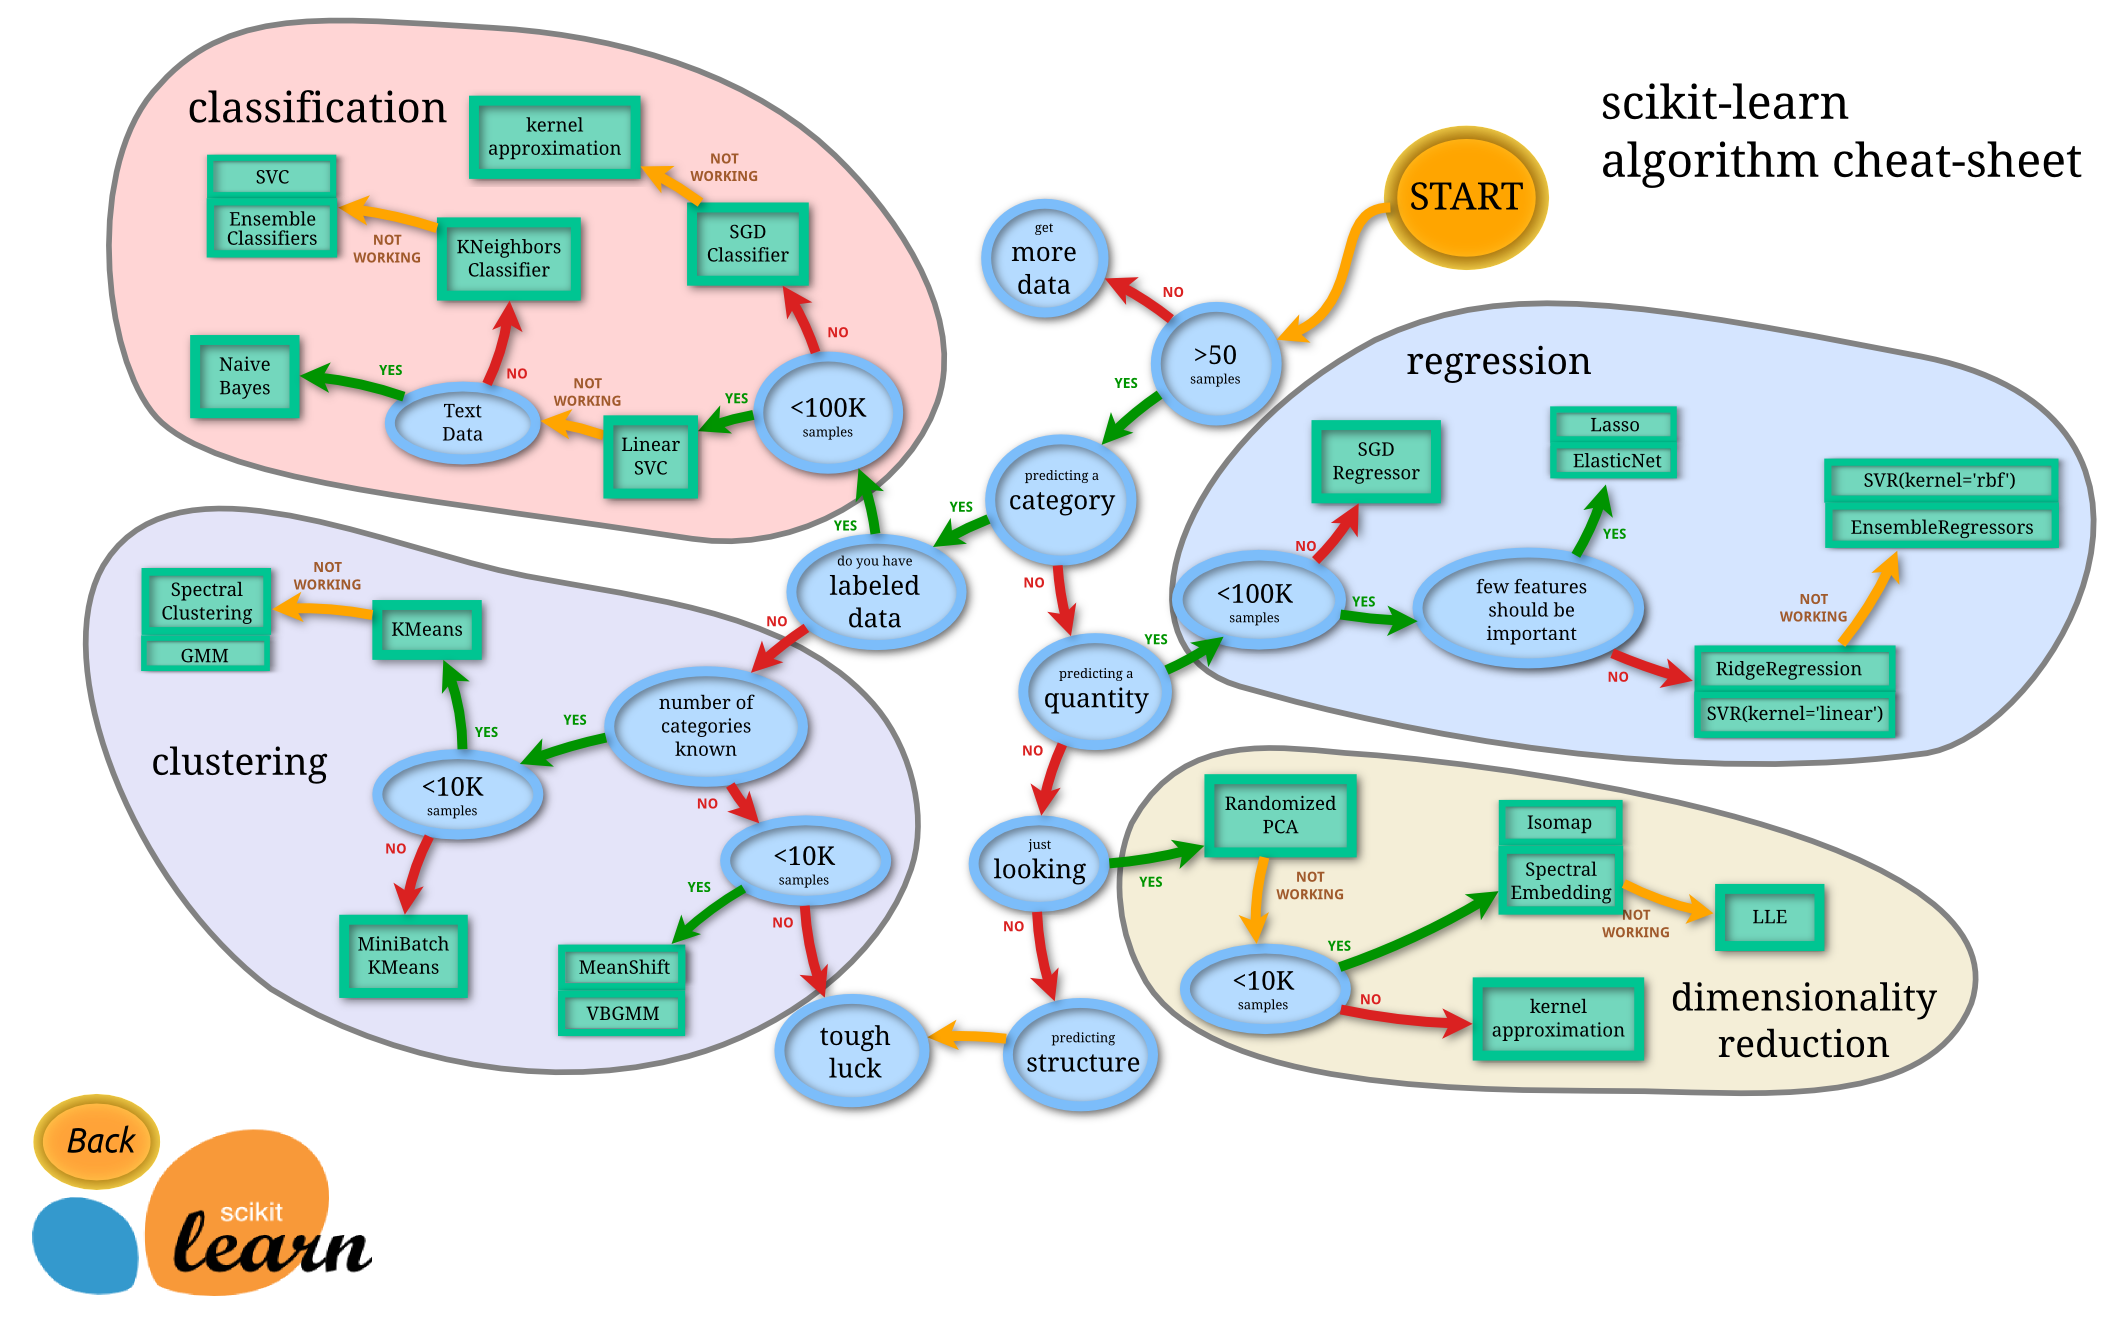
\includegraphics[
	width=0.65\textwidth
	]{images/FlowChartML.png}
	\caption{FlowChartML scikit-learn for any dataset which machine learning algortihm to choose}
	\label{fig:FlowChart}
\end{figure}
%explain the need for automation and then the boost of information, I try to give.

\subsection{research question}
% the proposed annotations
We base our research question on the work of Joaquin to give properties to algorithms\cite{Joaquin-phd}. More specifically we look more closely to the resilience properties and the bias-variance profile. 
Earlier research has been done on scalability and resilience to irrelevant variables\cite{Resil-1}

\begin{itemize}
	\item scalability: runtime is measured with either a varying sample size or varying feature space 
	\item robustness
\end{itemize}
The question for scalability is how varying sample size and feature space influences the runtime. Is there a measure to match this. 


%\subsection{thesis structure}


\subsection{Outline}
In the first chapter the research question is introduced. In the second chapter background information is discussed relevant for the research. In the third chapter the setup of the experiments is outlined with the input and output of executed experiments. The fourth chapter shows the results of the experiments
\newpage


\section{Preliminaries} \label{Chapter2}
Before we discuss in detail the solutions for the steps of our approach, this chapter provides
some background knowledge and definitions which are required for a good understanding of
the remainder of this thesis.
\subsection{Sklearn/scikit-learn library}
The scikit-learn library is based in Python and is made to make machine learning in python accessible and organized. 
All resources are open source and hosted on Github. 
%subsubsections for algorithms?

\subsubsection{KNeighborsClassifier}
In the scikit-learn library KNeighborsClassifier is an implementation of the k-nearest neighbors algorithm(k-NN). K-NN uses instance-based learning or non-generalizing learning. This means that during fitting no complete model is made but only the given feature set is stored in order of appearing in a tree for example. The k-NN uses as it names tells the nearest neighbors for calculation. The inputted feature set is traversed to find the nearest points and depending on the parameter k, an amount of k points is searched for. Depending on the class of the k neighbors the classification is vote is decided. The default metric for distance measuring is Euclidean distance another option is the Manhattan distance which is less accurate but needs less computing. To find the nearest points an option can be made between a ball tree, a kd-tree or a brute search. This can heavily influence the search time, depending on the amount and size of the input (features and instances) this can influence the prediction time heavily but will not influence predictive accuracy. The previously mentioned k parameter is an influencer for prediction quality—find source---


\subsubsection{GaussianNB}
GaussianNB is a naïve Bayes classifier implementation assuming the feature set is gaussian distributed \cite{Bayes}. For fitting the data, a partial fit function is used based on the work of Chan, Golub and LeVeque \cite{Sam-var}. This calculates the assumed means and variances of a gaussian distribution of the inputted feature set. Based on this distribution the prediction is made by filling in the maximum likelihood. The limited calculation needed for classification and prediction makes this one of the fastest algorithms. The only parameter of this classifier specifies the prior probabilities of the classes, which will when specified not be adjusted to the given input. 

\subsubsection{BernoulliNB}
BernoulliNB is a naïve Bayes classifier implementation assuming a Bernoulli distribution with Boolean like values \cite{NB-text}. The first step of this implementation is checking if the features are binary-valued, if any other data is found this input will be binarized. This setting can be disabled or reduced by a threshold for the input. Based on this Boolean model a smoothed version of the maximum likelihood is used for prediction. This classifier is mostly used in document classification as it can binary store occurrence useful for prediction class probability. 

\subsubsection{SVC-rbf}
SVC-rbf is a support vector classifier(SVC) implementation with a radial basis function. The radial basis function(rbf) is used to handle a large feature dimension, since the standard support vector machine splits the spaces with linearly lines computation grows too large for a large feature space \cite{SVN}. The fit time is already quadratic with the number of samples based on the implementation of libsvm\cite{SVM}. The fitting of a SVC will assign each example to one of two categories and will represent them in a dimension space mapped so there is a clear separation between the two categories. With the radial basis function this is with the distant from the points indicated by a separation area. Classifying a point is finding in which class area this point falls. For a multiclass problem this is done in pairs of two for all categories and then the most voted class is picked \cite{Multi-pair-coup}.%TODO ---hyperparameters--

\subsubsection{RandomForestClassifier}
RandomForestClassifier is an ensemble method of directive trees \cite{RDF}. During fitting a random forest classifier constructs directive trees on subsamples of the input data and averages the results for the result. These sub-samples are chosen randomly so the results can vary between runs on the same input. A directive tree is a decision tree classifier which splits the features on certain thresholds to decide on the type of class. This splitting of the data is either randomly or choosing the best split, to measure this split a criterion is used like Gini or entropy. The amount of splits, features and samples are also considered and can be inputted. 

\subsubsection{AdaBoost}
AdaBoost is an ensemble classifier that fits other classifiers and outputs the weighted results of those classifiers \cite{AdaBoost}. AdaBoost trains these other classifiers on previously misclassified results by increasing their influence this makes it heavily subjected to noisy data and outliers. The scikit-learn library uses the multi class AdaBoost-SAMME implementation from J. Zhu et al \cite{MadaB}. The solution of J. Zhu also solves the lack of multi-class solution of the weak learners (other classifiers) by extending the initial AdaBoost algorithm with a forward stage wise additive step. In this step a continual calculation of a loss function will output the prediction and in a two class case it reduces to the initial solution.

\subsubsection{SDGClassifier}
SDGClassifier is an incremental function to stochastic approximate the gradient descent of the input \cite{SGDClass}. It will iteratively minimize or maximize a set of differentiable functions, the input must fit these differentiable functions and this makes than an optimal input is with a mean of zero.  This makes the classifier sensitive to raw data as it performs optimally with sparse features. The iterative steps needed are bound by the inverse of the learning rate and a threshold value. The threshold value indicates what degree of slope indicates a near minimal or maxima. The learning rate is used to update the model in each iteration.

\subsubsection{GradientBoostingClassifier}
GradientBoost is an ensemble classifier that builds from weaker classifiers \cite{GradientBoost}. Like AdaboostClassifier it builds an additive model in a forward stage-wise fashion.  The weak classifiers used in the scikit-learn implementation are decision trees.  %TODO add\cite{Greedy-GBC}



\subsection{Definitions and abbreviations}
\subsubsection{Definitions}

\begin{tabular}{ p{0.20\linewidth} p{0.7437\linewidth} }
	
	algorithm & The process with a specified in and output that solves a problem\\ [1ex]
	
	
	annotations & Adjectives of something like a machine learning algorithms, examples can be robust or biased\\ [1ex]
	
	categorical & property of the features distribution and content of the feature in this case meaning seperate distinc classes, which have no numerical meaning, a unique number for each distinguished class\\ [1ex]
	
	class	 & categorical featueres consist of at least 2 classes\\ [1ex]
	
	datapoint & a datapoint is a single value of a feature. For example an instance has for all feature of a dataset a single datapoint.\\[1ex]
	
	dataset manipulation & like the word suggested is the manipulation of dataset like injecting std deviation or inserting random categories. Adding or removing; of  features or instances to the dataset also counts as it also influence duration and/or accuracy. \\ [1ex]
	
	dense matrix & most values in a matrix are different and fluctuate with each row or collumn.(non-zero)\\ [1ex]
	
	distribution & A distribution of a dataset is the probability distribution of that dataset. So considering the dataset what are the odss of picking a specific value. \\ [1ex]
	
	features & part of a whole, Consider a flower it can be the color, size, amount of branches, amount of leaves, age. Features describe someone or something in this context it describes something so you can make a prediction of the Target.\\ [1ex]
	
	fit & To fit the data, synonym with inputting the training data for preparing the algorithm for prediction\\ [1ex]
	
	Github & an online platfrom to host data. It uses git commands and is mostly used with programming project to organize a common project which each member can locally alter and centeralizly share updates or modifications. \\ [1ex]	
	
	machine learning algorithm & An algorithm that will will learn something and may adopt to the input to better fit the learned instance. To goal of learning can be mostly to predict a Target value, this can be part of an initial input.\\ [1ex]	
	
	numerical & exact values, more uniquely than a category. For example a temperature value or time value. Such a value can be subtracted or divided \\ [1ex]	
	
	profiling & To sketch information of something in a category, so you can relate it to other things in the same category\\ [1ex]
	
	robustness & \\ The ability of an algorithm to cope with changes in features. An algorithm is more robust if it deteriorates less than another.[1ex]	
	
	sample & the size of the to be predicted target set. So all distinct features once matched with a target feature\\ [1ex]
	
	scalability & is the capability of a system to handle growing amount of work. \\[1ex]
	
	sparse matrix & a matrix with lots of zero values, the counterpart of dense were all values fluctuate a lot.	\\ [1ex]
	
	target & In a classificication the value or classes that needs to be predicted, where it mostly about a single feature with at least 2 classes. This can be a feature of something \\ [+1ex]
	
	weight & The influence or power of a value, function or object. It can be expressed as a fraction of 1 to inidicate its factor from other weights.	\\ [1ex]
	
	
	
	
	
	
	algorithm & \\ [1ex]	
	\end{tabular}

\subsubsection{Abbreviations}
\begin{tabular}{ p{0.20\linewidth} p{0.7437\linewidth} }
	
	adaBoost & adaptive boosting algorithm \\
	
	biasVar & bias and variance \\
	
	SDG & Stochastic gradient descent \\
	
	std & standard deviation\\
	
	TU/e & Eindhoven University of Technology \\
	
	
\end{tabular}

\newpage
\section{Experimental setup} \label{Chapter3}
For different parts of the research different datasets are chosen. There is overlap between these datasets but the chosen datasets can have a large impact on shown results. Most results are shown as an average result of the datasets involved.
\subsection{Cross validation} \label{cross-val}
To easily test a single dataset once we use cross validation as it does this k times to get k splits of equal size. We can observe k classifications, to gain insight in duration time. We pick k=10 

\subsection{Bootstrapping} \label{motivation}
For the bias variance calculation it is import to gain multiple predictions for the same instance and with bootstrapping this can be easily achieved. The downside however can be an increased bias and reduced variance.

\subsection{Datasets} \label{description}
Depending on the property we are going to study we need different datasets or can make assumption. Classification features are not an optimal input for a nearest neighbor classifier as the distant between converted numbers does not tell much about the relation between the features. Multiple target classes datasets are inconvenient for the bias-variance calculation, so we focus on 2 class target datasets, which there are plenty enough on openml. 

\subsubsection{Bias-variance datasets}
An important part of a dataset to be viable for bias variance analysis is it having 2 classes as target due to calculation we use to find the bias and variance error. The bias and variance error is in this way like recall or precision error.  %give picture of instance versus features
\subsubsection{Categorical datasets}
Categorical datasets hold only features with categorical values
\subsubsection{Numerical datasets}
Numerical datasets hold only features with numerical values
\subsection{Collected data}
For each experiment data is saved to give insight to what the results are. Depending on the experiment different data is important or stored. 
\begin{itemize}
	\item predictive accuracy for measuring the predictive accuracy we store the default sklearn scoring calculation
	\item duration instances for the time needed to calculate 
	\item control
\end{itemize}
\subsubsection{Duration}
For each classification instance and for each prediction the time is added to indicate how the classification took. 

\subsubsection{Predictions}\label{pred}
For each predictions the outputted target value. Multiple files indicate multiple predictions. One of the files is also the true prediction of the inputted test set. 

\subsubsection{scores}
Gives the predictive accuracy of all the made classifiers. There can be multiple lists for each configuration of classifier or test input. The score is a value between 0 and 1 indicating the fraction of rightly predicted values

\subsubsection{SummaryGuesses}
SummaryGuesses give a quick overview of the obtained results. It stores in python dictonaries the total amount of predictions for each class. The results is that you can easily observe if a classifier has picked a class exclusively and you can compare the balance to the inputted dataset to see if the classifier does find a difference between classes. This data can also be generated from the predictions \ref{pred}.

\subsubsection{BiasVar}
When bootstrapping is done a bias and variance error is calculated together with the total error value. These are stored for easy lookup to the bias and variance error part of a classifier.

\subsubsection{Identifier}
The data input is shuffled as the saved datasets are sorted by class. The identifier can be used to match prediction results to a specific feature. This way of saving is used to reduce space needed to save potential useful information. Odd behavior on small datasets can be explained by an off balanced dataset for training. This cut of the data can be realistic but may affect averaged result significantly. 

\subsection{Experiments}
Experiments are grouped by all mentioned classifier with some initial settings on the dataset and/or classifiers. Experiments are defined as functions in python with input values indicating the way the experiment is done and on which dataset.
\subsubsection{Scalability}
Scalability experiments can be split up in instance based or features based. To measure the effect of features we take datasets with lots of features and remove features in steps to find the impact of these lost features. There is a disadvantage with this strategy as some classifiers calculate values like feature importance which depend on a somewhat complete dataset of features. The removed features are randomly chosen and can be defining features for the accuracy of the dataset. 
Another option  to measure scalability is to measure the impact of number of instances. For most classifiers each instance is considered during training and we measure an average calculation for each feature. The duration is measured over the whole dataset by doing a 10 fold cross validation.
%We compare the found scalability against the perceived running time upper or lower bounds. 

\subsubsection{Duplicate features}
Duplicate features experiments have multiple goals in mind. By adding existing feature we can measure scalability of datasets with some amount of features. These duplicate features can also be identified as adding little to the dataset or the same features can overrule existing important features. The accuracy on these modified dataset
can teach us about the impact of features on accuracy and how classifiers handle these irrelevant features. The method to add these duplicate features is by randomly picking and adding. This can result in features being multiple times in the manipulated  dataset even though it is only twice the orignal dataset size. The accuracy is measured over the whole dataset by doing a 10 fold cross validation.
\subsubsection{Random Features}
Random features experiments have similar goals in mind as duplicate features. By adding the random features we can measure scalability of datasets with randomish features. These random features can deceivingly have information as there is much variability. By measuring the accuracy we can observe what the impact is for different classifiers. There are two sorts of random features we add; Numerical and categorical features. We add either the categorical or numerical depending on the distribution of the dataset. The odds of either a categorical or numerical feature being added is the distribution of the initial dataset. The accuracy is measured over the whole dataset by doing a 10 fold cross validation. %\cite{catVSnum} the influence of categorical vs numerical why we need to add a similair feature.
 
\paragraph{categorical random features \newline}
The categorical random feature is a uniform value between 0 and k. The value of k can influence how a classifier perceive this random feature. For all the instances in the set a uniform random number between 0 and 1 is multiplied by k and then rounded. 
\paragraph{numerical random features \newline}
The numerical random feature is a uniform random value between 0 and 1. This feature has in this case all unique values.


\subsubsection{Noisy data}
Datasets can get more noisy over time. During training of a machine learning algorithm the dataset is clean and over time new data can change. By measuring the predictive accuracy off the algorithms on more noisy datasets the robustness can be measured. The accuracy is measured over the whole dataset by doing a 10 fold cross validation.

\paragraph{categorical features \newline}
To explain the implementation of our noisy data for a categorical feature we present this snippet of pseudo code. THe input is the dataset X and the amount of noise. The amount can be converted to a percentage of features being flipped by this formula $()1-1/(amount+0.5))*100$. The distribution$_X$ is derived from the dataset X as the probability distribution of all categorical classes in a feature. The random.choice function uses this probability function to pick a value in the range of the feature. The default random function picks a uniform random value between 0 and 1.  \\
Initiliaze distribution$_X$ for all features in dataset X\\
\textbf{for} numerical feature k in dataset X\\
.\hspace{1cm} \textbf{for} datapoint x in feature k\\
.\hspace{2cm} \textbf{if} random()*amount $>$ 0.5 \\	
.\hspace{3cm} x = random.choice(distribution$_X$ feature k) 
\\

\paragraph{numerical features \newline}
The input is the dataset X and the amount of noise. The amount is multiplied by the standard deviation to give the maximum deviation of the feature. The calculation for the std$_X$ is done beforehand to control the deviation for all datapoints in the feature set. The random function is like mentioned before producing a uniform random value between 0 and 1.\\
Calculate std$_X$ for all features in dataset X\\
\textbf{for} numerical feature k in dataset X\\
.\hspace{1cm} \textbf{for} datapoint x in feature k\\
.\hspace{2cm} \textbf{if} random() $>$ 0.5 \\	
.\hspace{3cm} x = x + random() *amount*(std$_X$ for feature k)\\
.\hspace{2cm} \textbf{else}  \\	
.\hspace{3cm} x = x - random() *amount*(std$_X$ for feature k) 
\\

\subsubsection{Bias Variance}
To measure the bias and variance error factor we use the calculation of Kohavi and Wolpert\cite{BiasCalc}. This is the same measure used in the work of Joaquin et al.\cite{Bias-var}. This experiment is made to reproduce that experiment with the scicikit-learn library. The input for the bias and variance calculation is done by doing 40 bootstraps. 
 
\section{Experimental Results} \label{Chapter4}


\subsection{Scalability}
All results with a duration axis. The duration axis is in seconds and shows a 10 fold cross validiation. This means that the duration encompasses 10 times fitting over 90\% of the data and 10 times predicting 10\% of the data.

\subsubsection{features}

\paragraph{Categorical features}
the averaged results are shown in figure \ref{fig:FeatAddCat}
\begin{figure}[h] %use t for top of page instead of h for here
	\centering
	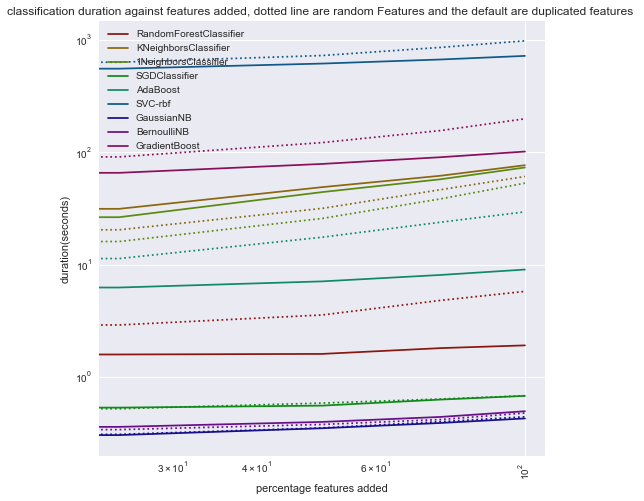
\includegraphics[
	width=0.65\textwidth
	]{images/scalability/FeatAddCat.png}
	\caption{Features added straight line represent duplicate features and dotted line are random categorical features between 0 and 2}
	\label{fig:FeatAddCat}
\end{figure}

\newpage
\paragraph{Numerical features}
in figure \ref{fig:FeatAddNonCat} and the slope in figure \ref{fig:FeatAddNonCatSlope}
\begin{figure}[h] 
	\centering
	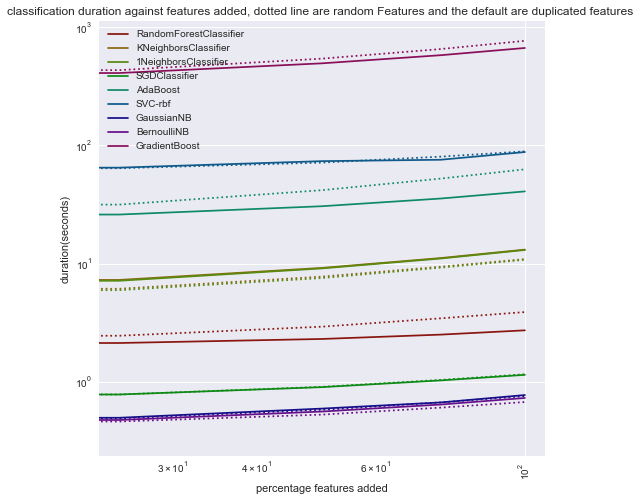
\includegraphics[
	width=0.65\textwidth
	]{images/scalability/FeatAddNonCat.png}
	\caption{Features added straight line represent duplicate features and dotted line are random numerical features}
	\label{fig:FeatAddNonCat}
\end{figure}


\begin{figure}[h] 
	\centering
	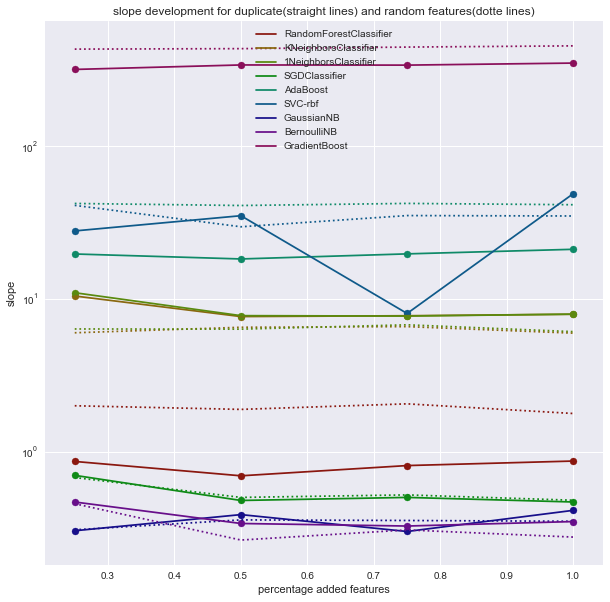
\includegraphics[
	width=0.65\textwidth
	]{images/scalability/FeatAddNonCatSlope.png}
	\caption{Features added straight line represent duplicate features and dotted line are random numerical features}
	\label{fig:FeatAddNonCatSlope}
\end{figure}
\newpage
\paragraph{combined}
in figures \ref{fig:FeatMan} and \ref{fig:FeatManLog} adding and removing features is shown.
in figures \ref{fig:FeatManSlope1Log},\ref{fig:FeatManSlope1} and \ref{fig:FeatManSlope}
\begin{figure}[h] 
	\centering
	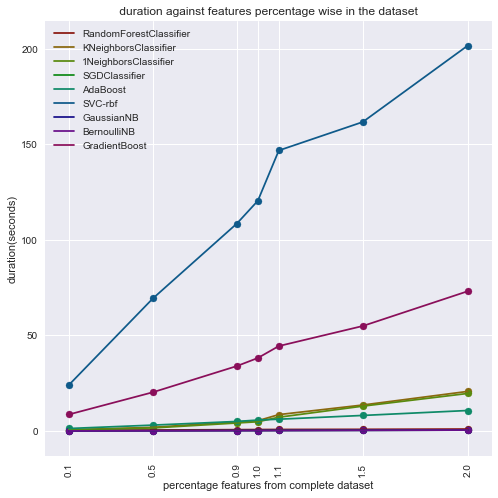
\includegraphics[
	width=0.65\textwidth
	]{images/scalability/FeatMan.png}
	\caption{features randomly removed and feature randomly duplicated}
	\label{fig:FeatMan}
\end{figure}

\begin{figure}[h] 
	\centering
	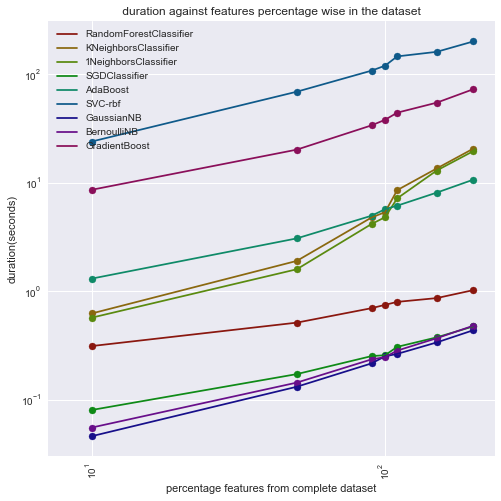
\includegraphics[
	width=0.65\textwidth
	]{images/scalability/FeatManLog.png}
	\caption{features randomly removed and feature randomly duplicated}
	\label{fig:FeatManLog}
\end{figure}

\begin{figure}[h] 
	\centering
	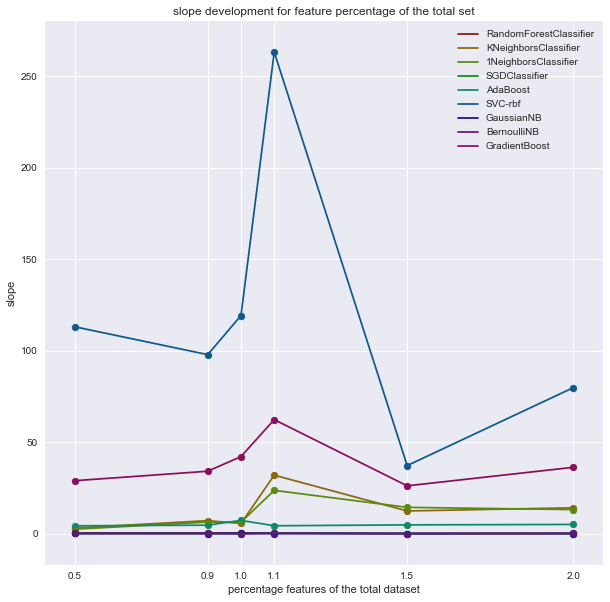
\includegraphics[
	width=0.65\textwidth
	]{images/scalability/FeatManSlope.png}
	\caption{features randomly removed and feature randomly duplicated}
	\label{fig:FeatManSlope}
\end{figure}

\begin{figure}[h] 
	\centering
	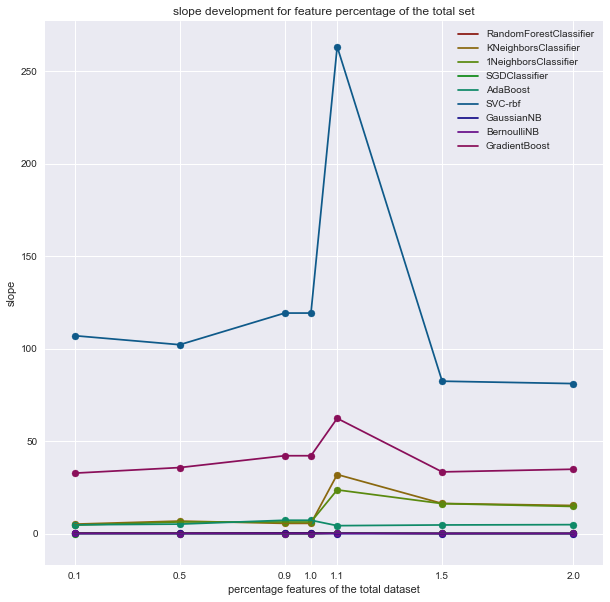
\includegraphics[
	width=0.65\textwidth
	]{images/scalability/FeatManSlope1.png}
	\caption{features randomly removed and feature randomly duplicated}
	\label{fig:FeatManSlope1}
\end{figure}

\begin{figure}[h] 
	\centering
	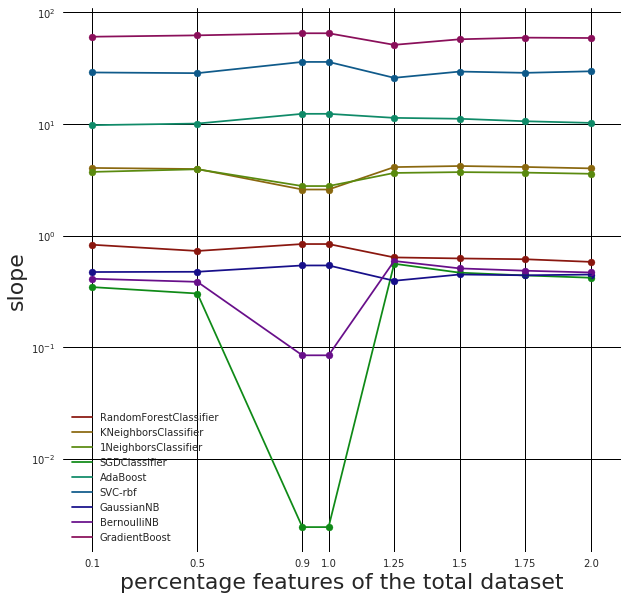
\includegraphics[
	width=0.65\textwidth
	]{images/scalability/FeatManSlope1Log.png}
	\caption{features randomly removed and feature randomly duplicated}
	\label{fig:FeatManSlope1Log}
\end{figure}


\newpage
\subsubsection{Instances}
\begin{figure}[h] 
	\centering
	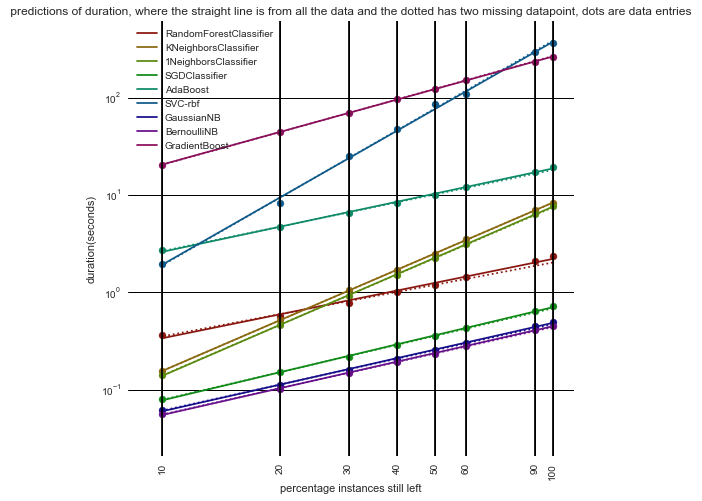
\includegraphics[
	width=0.65\textwidth
	]{images/scalability/Instances.png}
	\caption{splitting a dataset in parts}
	\label{fig:Instances}
\end{figure}

\begin{figure}[h] 
	\centering
	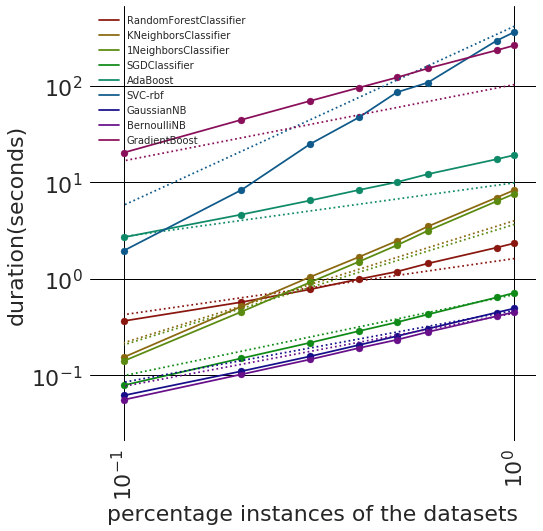
\includegraphics[
	width=0.65\textwidth
	]{images/scalability/InstancesPrediction.png}
	\caption{features randomly removed and feature randomly duplicated}
	\label{fig:InstancesPred}
\end{figure}
\newpage
\subsection{Redundant features}
We consider here both random and duplcite features as they are both redundant.


\subsection{Noisy data}
Datasets in these experiments get increasingly more random by injecting the features with noise.
\begin{figure}[h] 
	\centering
	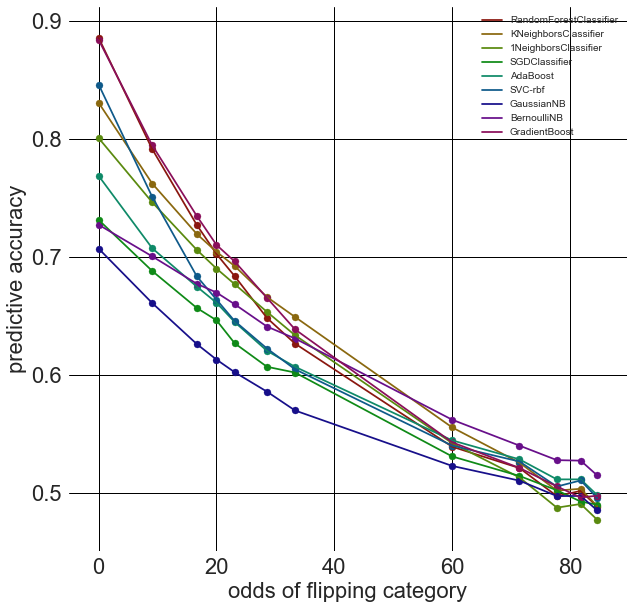
\includegraphics[
	width=0.65\textwidth
	]{images/NoisyFeatures/predCatFeat.png}
	\caption{flipping categories for categorical features}
	\label{fig:predCatFeat}
\end{figure}

\begin{figure}[h] 
	\centering
	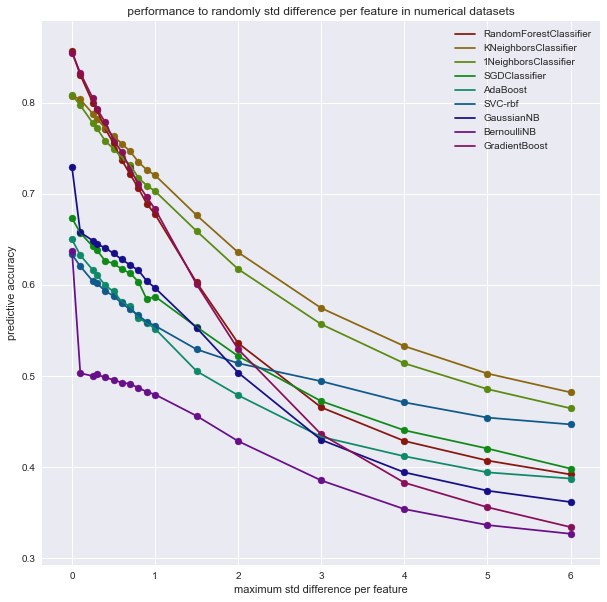
\includegraphics[
	width=0.65\textwidth
	]{images/NoisyFeatures/predNonCatFeat.png}
	\caption{adding or removing uniformly random std to numerical features}
	\label{fig:predNonCatFeat}
\end{figure}

\begin{figure}[h] 
	\centering
	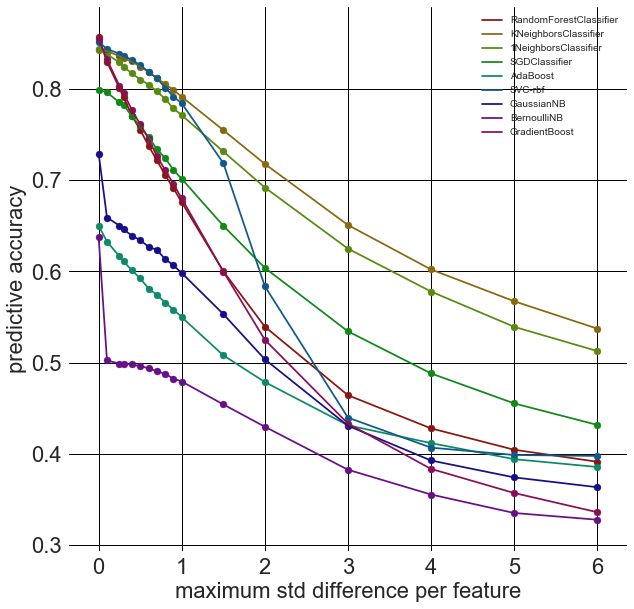
\includegraphics[
	width=0.65\textwidth
	]{images/NoisyFeatures/predNonCatFeatPre.png}
	\caption{adding or removing uniformly random std to numerical features and preprocessing for some algorithms.}
	\label{fig:predNonCatFeat}
\end{figure}


\subsection{Bias variance}


\subsection{Ontology}
To present the results from all the experiments, this ranks the different algorithms on different aspects discussed.
The result will be a ranking of algorithms on different scales. The scales are:
\begin{itemize}
	\item training and prediction duration
	\item robustness to noise
	\item preprocessing needed
	\item initial prediction accuracy
\end{itemize} 

\section{Discussion} \label{Chapter5}

\subsection{Resilience to noise}



\subsubsection{different approach}
Instead of measuring the influence of standard deviation, we tried to add standard values to all features, the problem with that is features have different deviation and some classifiers prefer a zero mean. The results were similair to injection std but more abrupt. Just changing(moving/word) all features for some datasets mend a drop in accuracy but the continuation of upping the number mend little to change accuracy further.


\subsection{MetaFeatures}
Meta features like mean mutual information or entropy for categorical features are calculated for our enhanced dataset with duplicate feature and random features. The result is that they do little to change these values and so do not indicate reduced information even tough commonly the results deteriorate when these features are added. However if we take the adjusted mean mutual information we can see a more clearer distinction between the permutations of the datasets. With those values the noisy dataset can be more recognized as being worse than before. The normalized  is combination of both which has all three kinds in some case the best or the worsed.

The calculation of the normalized:
$sqrt(H(labels_true) * H(labels_pred))$


the calculation for two cluster for adjusted mean mutual information:
$AMI(U, V) = [MI(U, V) - E(MI(U, V))] / [max(H(U), H(V)) - E(MI(U, V))]$


The default mutual information is:
$MI(U,V) = \sum_{i = 1}^{I} U \mid\sum_{j = 1}^{I} V \mid \dfrac{\mid U_i \cap V_j\mid}{N} $log $\dfrac{N\mid U_i \cap V_j\mid}{\mid U_i\mid \mid V_j\mid}$
% Misschien een tabel maken en verschil laten zien

\begin{figure}[H]
	\centering
	\begin{subfigure}[b]{0.45\textwidth}
		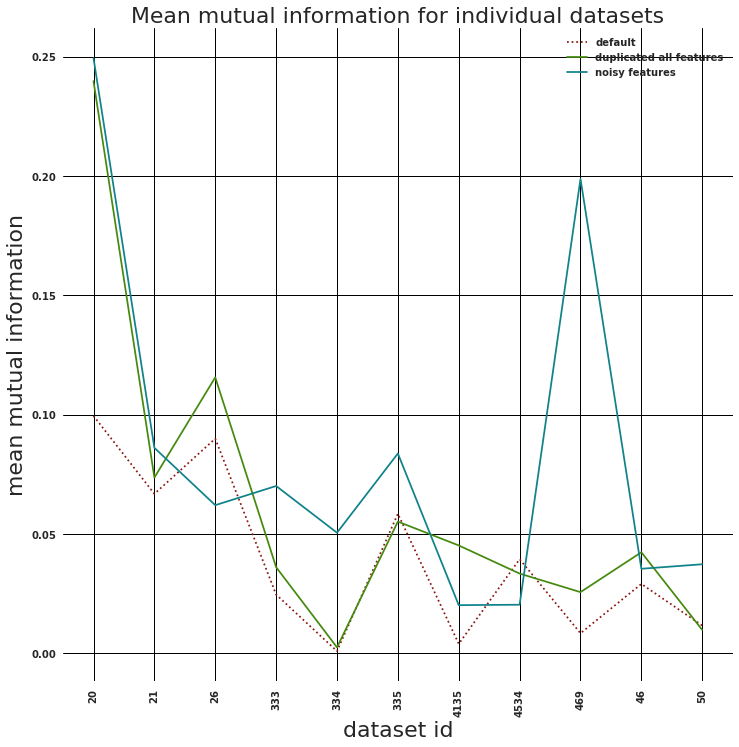
\includegraphics[width=\textwidth]{images/MeanMutualInformation.png}
		\caption{Mean Mutual Information for mututations of datasets}
		\label{fig:MMI}
	\end{subfigure}
	\begin{subfigure}[b]{0.45\textwidth}
		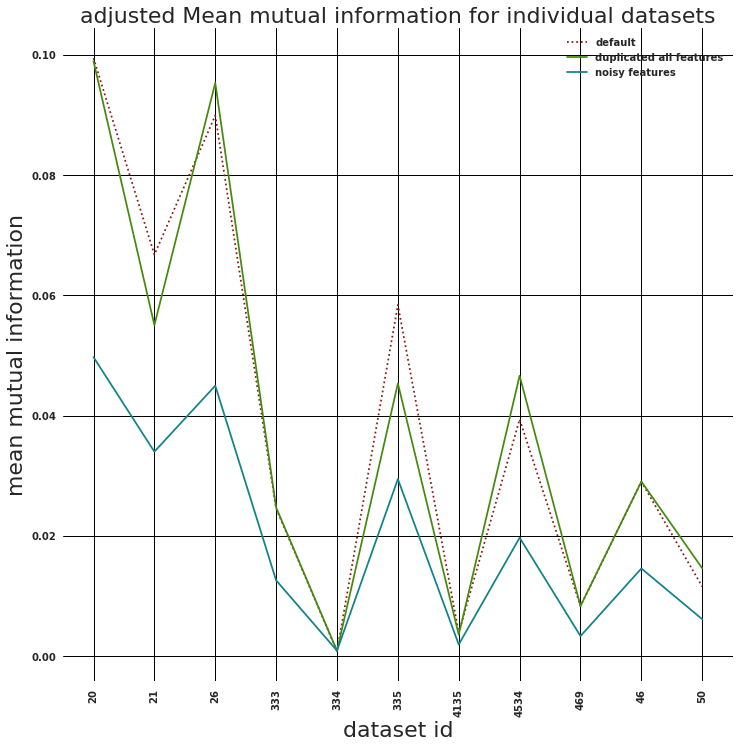
\includegraphics[width=\textwidth]{images/adjustedMeanMutualInformation.png}
		\caption{adjusted Mean Mutual Information for mututations of datasets}
		\label{fig:AMMI}
	\end{subfigure}
	\begin{subfigure}[b]{0.45\textwidth}
		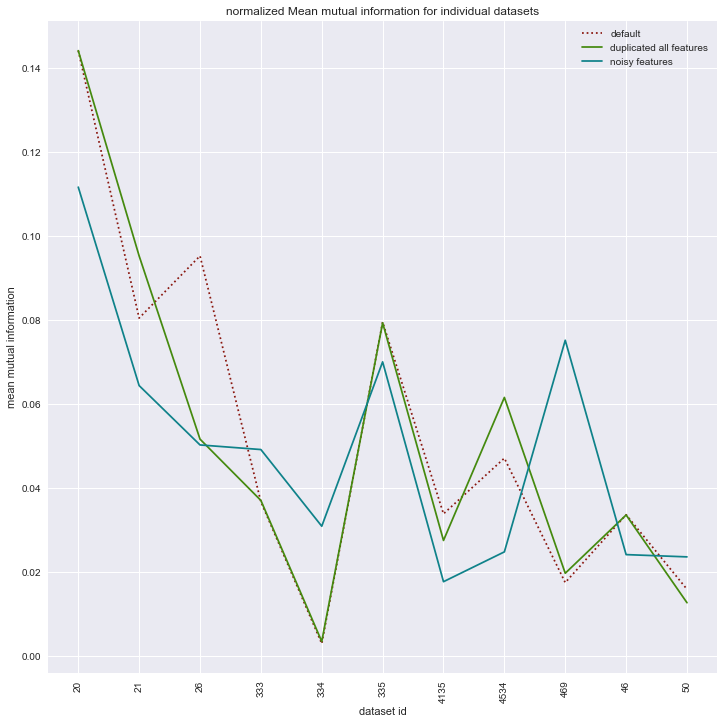
\includegraphics[width=\textwidth]{images/normalizedMeanMutualInformation.png}
		\caption{normalized Mean Mutual Information for mututations of datasets}
		\label{fig:NMMI}
	\end{subfigure}
	\caption{Check-out times}\label{fig:MMIs}
\end{figure}


\newpage
\section{Conclusion} \label{Chapter6}
\subsection{replication of previous work}

\subsection{New discoveries}




\subsection{Future work}
\subsubsection{More computation}
with more computation time we can further solidify the results or see a different approach

Use datasets outside of openml like keggle%cite
to illistrate that openml is not the factor, openml can be focused on a certain subgroup more than another 

splitting datasets for finer results. By focusing on a certain dataset type you can find why that dataset type is robust, think about sparse/dense feature rich, feature less. A combination.





\section{References}
\begingroup
\begin{thebibliography}{9}
\bibitem{Data-science} The Popularity of Data Science Software, Robert A. Muenchen, r4stats.com, (2017)
\bibitem{python-pop} Most Popular Programming Languages For Machine Learning And Data Science,Adarsh Verma, fossbytes.com, (2016)
\bibitem{ML-trends} 
Machine learning: Trends, perspectives, and prospects, M. I. Jordan, T. M. Mitchell, Science Volume 349 issue 6245 pages 255-260, (2015)
\bibitem{Big-data} Storage predictions: Will the explosion of data in 2017 be repeated in 2018?, Nick Ismail, www.information-age.com/, (2017)
\bibitem{Joaquin-phd} Understanding Machine Learning Performance with experiment databases, Joaquin Vanschoren, KU Leuven, (2010)
\bibitem{Resil-1} Quantifying the resilience of inductive classification algorithms, M. Hilario, A. Kalousis, 
Proceedings of the 4th European Conference on Principles of data mining and knowledge discovery, pages 106-115, (2000)
\bibitem{Sam-var}Updating Formulae and a Pairwise Algorithm for Computing Sample Variances Tony F. Chan* Gene H. Golub’* Randall J. LeVeque, Stanford CS tech report STAN-CS-79-773(1979)
\bibitem{SVM}LIBSVM: A library for support vector machines, Chang, Chih-Chung, Lin, Chih-Jen, ACM Transactions on Intelligent Systems and Technology (2011)
\bibitem{Multi-pair-coup} Probability estimates for multi-class classification by pairwise coupling, Wu, Lin, Weng, Journal of Machine Learning Research 5 (2004)
\bibitem{SVN} Support-Vector networks, Cortes, Corinna, Vapnik, Vladimir, Machine Learning Volume 20 issue 3 (1995)
\bibitem{Bayes} Idiot’s Bayes—Not So Stupid After All?, David J. Hand, Keming Yu, International Statistical Review Volume 69 Number 3(2001)
\bibitem{NB-text} A Comparison of event models for naïve Bayes text classification, Andrew McCallum, Kamal Nigam, AAAI-98 workshops on learning for text categorization (1998)
\bibitem{KNNreg} An introduction to kernel and nearest-neighbor nonparametric regression, N. S. Altman, American Statistician 46(3): 175-185 (1992)
\bibitem{RDF} Random Decision Forests, Tin Kam Ho, Proceedings of the 3rd Iternational Conference on Document analysis and recognition (1995)
\bibitem{AdaBoost} A short introduction to Boosting, Yoav Freund, Robert E. Shapire, Journal of Japanse Society for artificial Intelligence 14(5):771-780 (1999)
\bibitem{MadaB} Multi-class AdaBoost, J. Zhu, S. Rosset, H. Zou, T. Hastie, Statistics and its Interface volume 2, pages 349-360 (2009)
\bibitem{SGDClass} Solving Large Scale Linear Prediction problems using stochastic gradient descent algorithms, T. Zhang, ICML Proceedings of the 21 International conference on machine learning (2004)
\bibitem{GradientBoost} Stochastic Gradient Boosting, J. H. Friedman,  Computational Statistics \& Data analysis – Nonlinear methods and data mining volume 38 issue 4 pages 367-378,(2002)
\bibitem{Greedy-GBC} Greedy function approximation: A gradient boosting machine, J. H. Friedman, The annals of statistics volume 29 issue 5, pages 1189-1232,(2001)
Previous bias-variance research has shown a trend of larger dataset increasing the bias component but still fluctuating with  less than 10000 instances.
\bibitem{Bias-var} Experiment databases, J. Vanschoren, H. Blockeel, B. Pfahringer, G. Holmes, Machine Learning Volume 82 issue 2 pages 127-158, (2012)
\bibitem{BiasCalc} Bias plus variance decomposition for zero-one loss functions,R. Kohavi, D. Wolpert, Proceedings of the international conference on machine learning pages 275-283,(1996)


 
     
\end{thebibliography}
\endgroup

\section{Appendix}
\subsection{datasets per figure}
%insert tables

\end{document}